\section{Lab: Multithreading}

\subsection{实验目的}
本实验旨在进一步了解多线程编程,在操作系统中实现线程执行和切换等操作。实验将在用户级线程包中实现线程之间的切换,使用多个线程来加速程序,并实现barrier。

\subsection{实验步骤}
\subsubsection{实现用户线程切换}
\begin{enumerate}
    \item 修改uthread.c文件:
          \begin{itemize}
              \item 添加一个context结构体保存线程上下文的寄存器。
                    \begin{lstlisting}[language=c,title=context结构体]
    struct context
    {
        uint64 ra;
        uint64 sp;

        uint64 s0;
        uint64 s1;
        uint64 s2;
        uint64 s3;
        uint64 s4;
        uint64 s5;
        uint64 s6;
        uint64 s7;
        uint64 s8;
        uint64 s9;
        uint64 s10;
        uint64 s11;
    };
    \end{lstlisting}
              \item 在thread结构体中添加一个保存上下文的context结构体成员。
                    \begin{lstlisting}[language=c,title=对thread结构体的修改]
    struct thread
    {
        char stack[STACK_SIZE]; 
        int state;              
        struct context context; /* 线程上下文 */
    };
        \end{lstlisting}

              \item 修改thread\_schedule函数实现线程切换。
                    \begin{lstlisting}[language=c,title=对thread\_schedule函数的修改]
    void thread_schedule(void)
    {
        struct thread *t, *next_thread;
    
        ...
    
        if (current_thread != next_thread)  // 如果需要切换线程
        {
            next_thread->state = RUNNING;  // 设置下一个线程为运行状态
            t = current_thread;  // 保存当前线程
            current_thread = next_thread;  // 切换到下一个线程
            // 切换线程上下文
            thread_switch((uint64)&t->context, (uint64)&next_thread->context);  
        }
        else
            next_thread = 0;  // 如果没有切换线程,则将next_thread置为0
    }            
              \end{lstlisting}
              \item 修改thread\_create函数初始化context结构体,设置栈顶指针和函数指针。
                    \begin{lstlisting}[language=c,title=对thread\_create函数的修改]
    void thread_create(void (*func)())
    {
        struct thread *t;

        for (t = all_thread; t < all_thread + MAX_THREAD; t++)  // 查找空闲的线程结构
        {
            if (t->state == FREE)  // 如果找到空闲线程
                break;  // 跳出循环
        }
        t->state = RUNNABLE;  // 设置线程状态为可运行

        //添加的部分
        t->context.sp = (uint64)&t->stack + STACK_SIZE;  // 初始化线程栈顶指针
        t->context.ra = (uint64)func;  // 设置返回地址为函数指针
    }
            \end{lstlisting}
          \end{itemize}

    \item 修改uthread\_switch.S文件,实现thread\_switch函数,保存当前线程的寄存器并恢复新线程的寄存器。
          \begin{lstlisting}[language={[x86masm]Assembler},title=实现thread\_switch汇编]
        thread_switch:
            sd ra, 0(a0)
            sd sp, 8(a0)
            sd s0, 16(a0)
            sd s1, 24(a0)
            sd s2, 32(a0)
            sd s3, 40(a0)
            sd s4, 48(a0)
            sd s5, 56(a0)
            sd s6, 64(a0)
            sd s7, 72(a0)
            sd s8, 80(a0)
            sd s9, 88(a0)
            sd s10, 96(a0)
            sd s11, 104(a0)
            ld ra, 0(a1)
            ld sp, 8(a1)
            ld s0, 16(a1)
            ld s1, 24(a1)
            ld s2, 32(a1)
            ld s3, 40(a1)
            ld s4, 48(a1)
            ld s5, 56(a1)
            ld s6, 64(a1)
            ld s7, 72(a1)
            ld s8, 80(a1)
            ld s9, 88(a1)
            ld s10, 96(a1)
            ld s11, 104(a1)
            ret    /* return to ra */
        \end{lstlisting}
\end{enumerate}

\subsubsection{使用 UNIX pthread 线程库实现一个线程安全的哈希表}
这部分实现不需要使用xv6操作系统部分的代码。首先观察ph.c文件,编译运行,发现程序在单线程运行时,哈希表没有出现丢失key的情况,而在双线程运行时就会发生丢失key的情况。经过观察,发现put函数中的插入操作不是线程安全的,通过为这部分代码加入互斥锁便可解决问题。

\begin{enumerate}
    \item 在全局变量中加入一个互斥锁。
          \begin{lstlisting}[language=c,title=声明互斥锁]
    struct entry *table[NBUCKET];
    int keys[NKEYS];
    int nthread = 1;
    // 添加的互斥锁
    pthread_mutex_t lock[NBUCKET];
    \end{lstlisting}
    \item 在main函数的开头初始化互斥锁。
          \begin{lstlisting}[language=c,title=初始化互斥锁]
    int main(int argc, char *argv[])
    {
        ...
    
        for (int i = 0; i < NBUCKET; i++)
        {
            pthread_mutex_init(&lock[i], NULL);
        }
    
        ...
    }
    \end{lstlisting}
    \item 在put函数中使用互斥锁,确保线程安全。
          \begin{lstlisting}[language=c,title=对put函数的修改]
    static void put(int key, int value)
    {
        int i = key % NBUCKET;

        // is the key already present?
        struct entry *e = 0;
        for (e = table[i]; e != 0; e = e->next)
        {
            if (e->key == key)
                break;
        }
        if (e)
        {
            // update the existing key.
            e->value = value;
        }
        else
        {
            // 添加互斥锁
            pthread_mutex_lock(&lock[i]);
            insert(key, value, &table[i], table[i]);
            pthread_mutex_unlock(&lock[i]);
        }
    }
    \end{lstlisting}
\end{enumerate}

\subsubsection{实现barrier}
barrier 函数的作用是在并发编程中同步多个线程,使得它们在某个点上等待,直到所有线程都到达该点,然后再继续执行。这确保了所有线程在某个阶段结束前不会提前进入下一个阶段。

\begin{lstlisting}[language=c,title=对barrier函数的实现]
    static void barrier() 
    {
        pthread_mutex_lock(&bstate.barrier_mutex);  // 加锁保护屏障状态

        bstate.nthread++;  // 已到达屏障的线程数加1

        if (bstate.nthread == nthread) 
        {  // 如果所有线程都到达屏障
            bstate.nthread = 0;  // 重置已到达线程数
            bstate.round++;  // 增加屏障轮次
            pthread_cond_broadcast(&bstate.barrier_cond);  // 唤醒所有等待线程
        } 
        else 
        {
            // 等待其他线程到达屏障
            pthread_cond_wait(&bstate.barrier_cond, &bstate.barrier_mutex);  
        }

        pthread_mutex_unlock(&bstate.barrier_mutex);  // 解锁
    }

\end{lstlisting}

\subsection{评测结果}
利用grade-lab-thread脚本评测,得到结果如图\ref{fig:thread}所示。
\begin{figure}[h]
    \centering
    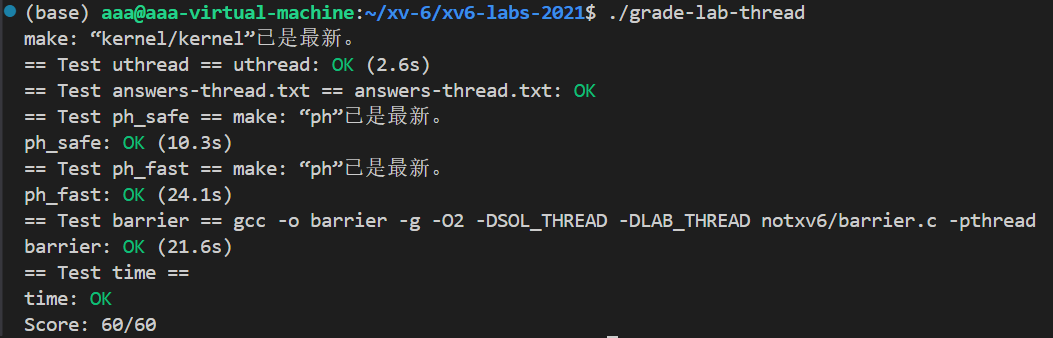
\includegraphics[width=\linewidth]{pics/thread评测结果.png}
    \caption{评测结果}
    \label{fig:thread}
\end{figure}

\subsection{实验小结}

\subsubsection*{为什么使用单线程运行哈希表就不会丢失key,而双线程就会丢失?}
有两个线程时,缺失键的问题是因为存在竞态条件。多个线程同时访问和修改共享数据(哈希表)时,会导致不可预测的结果。例如,线程1和线程2同时检查同一个桶,并发现键不存在,随后都尝试插入该键,这会导致其中一个插入操作被覆盖,从而导致缺失键。使用互斥锁(mutex)来保护对哈希表的访问可以解决这个问题。
\subsubsection*{总结}
本次实验深入探讨了多线程编程的实现与应用,涵盖了用户级线程切换、线程安全数据结构以及同步机制的实现。通过这些实现,我们不仅掌握了多线程编程的基本技术,还理解了线程同步和数据一致性的重要性。这些技能对于开发高效、可靠的并发程序具有重要意义。本实验为将来的复杂系统开发奠定了坚实基础。